\documentclass[aspectratio=1610,handout]{beamer}
\usepackage[fontset=fandol]{ctex}
%\usepackage{fontspec}
\usepackage[T1]{fontenc}
%\usefonttheme{serif}
\usefonttheme[onlymath]{serif}

% other packages
\usepackage{latexsym,amsmath,xcolor,multicol,booktabs,calligra}
\usepackage{graphicx,pstricks,listings,stackengine}
\usepackage{
	bm,
	mathrsfs,
	xparse,
	%esint,
	physics2,
	pgfplots,
	mathrsfs,
	perpage,
	ulem,
	amsthm,
	geometry,
	upgreek,
	%mathptmx,
	%txfonts,
	lmodern,
	gbt7714,
	subcaption,
	booktabs,
	cases,
	tcolorbox,
	tabularx,
	longtable,
    xcolor,
    fixdif,
    derivative,
    subcaption
}

\usepackage{hyperref}


\pgfplotsset{compat=1.15}
\usetikzlibrary{arrows,arrows.meta}
\definecolor{uuuuuu}{rgb}{0.26666666666666666,0.26666666666666666,0.26666666666666666}

\usephysicsmodule{ab,ab.legacy,diagmat}

\makeatletter
\newcommand\vb{\@ifstar\boldsymbol\mathbf}
\newcommand\va[1]{\@ifstar{\vec{#1}}{\vec{\mathrm{#1}}}}
\newcommand\vu[1]{%
\@ifstar{\hat{\boldsymbol{#1}}}{\hat{\mathbf{#1}}}}
\makeatother

\newcommand\bmqty[1]{\begin{bmatrix}#1\end{bmatrix}}
\newcommand\pmqty[1]{\begin{pmatrix}#1\end{pmatrix}}

\usetikzlibrary{angles,quotes,patterns,decorations.markings,arrows.meta}

\hypersetup{bookmarks=true,bookmarksopen=false,pdfstartview=FitV}

\DeclareSymbolFont{EulerExtension}{U}{euex}{m}{n}
\DeclareMathSymbol{\euintop}{\mathop} {EulerExtension}{"52}
\DeclareMathSymbol{\euointop}{\mathop} {EulerExtension}{"48}
\let\intop\euintop
\let\ointop\euointop

\newcommand{\im}{\mathrm{i}}
\newcommand{\ex}[1]{\mathrm{e}^{#1}}
\newcommand{\avg}[1]{\left\langle{#1}\right\rangle}
\DeclareMathOperator{\res}{res}
\newcommand{\dotv}[1]{\dot{\vb*{#1}}}
\newcommand{\alarm}[1]{\textcolor{red}{#1}}

% --- Custom commands for Chinese template ---
\newcommand{\en}[1]{\textenglish{\small (#1)}} % English annotation in Chinese context
\newcommand{\highlight}[1]{\alert{#1}} % Highlight text

%\ctexset{today=big}

\author[你的名字]{\Large 你的名字}
\title{WHU Beamer 模板演示与使用指南}
\subtitle{武汉大学风格 Beamer 主题}
\institute[你的学校/机构]{\small 你的学校/机构\\[8pt]
    专业 / 年级}
\date{\today}
\usepackage{whu}

\hypersetup{pdftitle={WHU Beamer 模板演示},pdfauthor={}}

% defs
\def\cmd#1{\texttt{\color{red}\footnotesize $\backslash$#1}}
\def\env#1{\texttt{\color{blue}\footnotesize #1}}
\definecolor{deepblue}{rgb}{0,0,0.5}
\definecolor{deepred}{rgb}{0.6,0,0}
\definecolor{deepgreen}{rgb}{0,0.5,0}
\definecolor{halfgray}{gray}{0.55}

\lstset{
    basicstyle=\ttfamily\small,
    keywordstyle=\bfseries\color{deepblue},
    emphstyle=\ttfamily\color{deepred},    % Custom highlighting style
    stringstyle=\color{deepgreen},
    numbers=left,
    numberstyle=\small\color{halfgray},
    rulesepcolor=\color{red!20!green!20!blue!20},
    frame=shadowbox,
}

\setbeamertemplate{background}{
\includegraphics[width=\paperwidth,height=\paperheight]{images/background_1610.png}}
% bg-image 是背景图片名称，亲测 png、pdf 和 jpg 可行，eps 不行


\begin{document}

\kaishu
\begin{frame}
    \titlepage
    \begin{figure}[htpb]
        \begin{center}
            
\includegraphics[width=0.13\linewidth]{pic/whulogo+.png}
        \end{center}
    \end{figure}
\end{frame}

\begin{frame}
    \frametitle{目录}
    \tableofcontents%[sectionstyle=show,subsectionstyle=show/shaded/hide,subsubsectionstyle=show/shaded/hide]
\end{frame}

% --- Section 1: 快速开始 ---
\section{快速开始}

\begin{frame}{模板简介}{什么是 WHU Beamer 模板？}
    \begin{itemize}
        \item 这是一个基于 \textbf{武汉大学 (WHU)} 视觉风格的 Beamer 学术演示模板。
        \item 修改自 \href{https://github.com/xinchen13/WHU-Beamer-Theme}{\texttt{xinchen13/WHU-Beamer-Theme}}。
        \item 背景图片来自 \href{https://github.com/hrtan99/WHU-Beamer}{\texttt{hrtan99/WHU-Beamer}}。
        \item 配色方案采用武大官方「珞珈绿」(\texttt{whucolor})。
        \item 支持 \textbf{16:10} 和 \textbf{16:9} 两种屏幕比例。
        \item 同时提供\highlight{英文版}（\texttt{Slide.tex}），不含中文依赖。
    \end{itemize}
\end{frame}

\begin{frame}[fragile]{模板简介}{快速上手}
    \begin{enumerate}
        \item 在导言区修改个人信息：
        \begin{lstlisting}[language=TeX]
\author[你的名字]{\Large 你的名字}
\title{你的演示标题}
\subtitle{副标题}
\institute[你的学校]{你的学校/机构\\ 专业/年级}
\date{\today}
        \end{lstlisting}
        \item 在 \verb|\begin{document} ... \end{document}| 中添加内容。
        \item 用 \textbf{xelatex} 编译：
        \begin{lstlisting}[language=bash]
xelatex Slide-zh.tex
bibtex Slide-zh
xelatex Slide-zh.tex
xelatex Slide-zh.tex
        \end{lstlisting}
    \end{enumerate}
\end{frame}

% --- Section 2: 模板功能演示 ---
\section{模板功能演示}

\begin{frame}{模板功能演示}{基本块环境}
    \begin{block}{普通块 (block)}
        这是标准的 \texttt{block} 环境，用于一般内容展示。
    \end{block}
    \pause
    \begin{alertblock}{警告块 (alertblock)}
        这是 \texttt{alertblock} 环境，用于\highlight{强调重要信息}。
    \end{alertblock}
    \pause
    \begin{exampleblock}{示例块 (exampleblock)}
        这是 \texttt{exampleblock} 环境，用于展示示例。
    \end{exampleblock}
\end{frame}

\begin{frame}{模板功能演示}{分栏布局}
    \begin{columns}[T]
        \begin{column}{0.5\textwidth}
            \begin{block}{左栏}
                \begin{itemize}
                    \item 项目一
                    \item 项目二
                    \item 项目三
                \end{itemize}
            \end{block}
        \end{column}
        \begin{column}{0.5\textwidth}
            \begin{block}{右栏}
                \begin{enumerate}
                    \item 第一点
                    \item 第二点
                    \item 第三点
                \end{enumerate}
            \end{block}
        \end{column}
    \end{columns}
\end{frame}

\begin{frame}{模板功能演示}{图片插入}
    \begin{columns}[T]
        \begin{column}{0.5\textwidth}
            \begin{itemize}
                \item 用 \cmd{includegraphics} 插入图片。
                \item 支持格式：\texttt{png}, \texttt{pdf}, \texttt{jpg}。
                \item 图片放在 \texttt{images/} 或 \texttt{pic/} 文件夹。
            \end{itemize}
        \end{column}
        \begin{column}{0.5\textwidth}
            \centering
            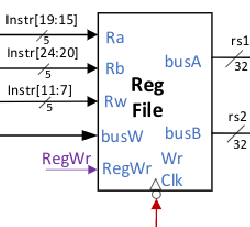
\includegraphics[width=0.8\linewidth]{pic/demo.png}
            \captionof{figure}{示例图片 (\texttt{pic/demo.png})}
        \end{column}
    \end{columns}
\end{frame}

\begin{frame}{模板功能演示}{数学公式}
    模板内置了常用的数学命令：
    \begin{itemize}
        \item \cmd{vb\{x\}} 粗体向量：$\vb{x}$, $\vb*{x}$
        \item \cmd{va\{x\}} 箭头向量：$\va{x}$, $\va*{x}$
        \item \cmd{vu\{x\}} 单位向量：$\vu{x}$, $\vu*{x}$
        \item \cmd{bmqty}, \cmd{pmqty} 矩阵：$\bmqty{a & b \\ c & d}$
        \item \cmd{im} 虚数单位，\cmd{ex\{x\}} 指数函数
        \item \cmd{avg\{x\}} 期望值：$\avg{x}$
        \item \cmd{highlight\{x\}} 高亮文本
        \item \cmd{en\{x\}} 英文标注\en{English annotation}
    \end{itemize}
\end{frame}

% --- Section 3: 自定义指南 ---
\section{自定义指南}

\begin{frame}[fragile]{自定义指南}{更换背景图片}
    \begin{itemize}
        \item 背景图片在导言区设置：
        \begin{lstlisting}[language=TeX]
\setbeamertemplate{background}{
  
\includegraphics[width=\paperwidth,
                    height=\paperheight]
  {images/background_1610.png}
}
        \end{lstlisting}
        \item 提供了两种比例的背景：
        \begin{itemize}
            \item \texttt{images/background\_1610.png} —— 16:10
            \item \texttt{images/background\_169.png} —— 16:9
        \end{itemize}
        \item 封面背景也已提供：
        \begin{itemize}
            \item \texttt{images/background\_cover\_1610.png}
            \item \texttt{images/background\_cover\_169.png}
        \end{itemize}
    \end{itemize}
\end{frame}

\begin{frame}[fragile]{自定义指南}{切换屏幕比例}
    \begin{itemize}
        \item 修改文档类选项：
        \begin{lstlisting}[language=TeX]
\documentclass[aspectratio=1610]{beamer}  % 16:10
\documentclass[aspectratio=169]{beamer}   % 16:9
        \end{lstlisting}
        \item 别忘了同步更换背景图片路径！
        \item 可去掉 \texttt{handout} 选项来启用演示模式（逐页展开）。
    \end{itemize}
\end{frame}

% --- Section 4: 致谢与许可 ---
\section{致谢与许可}

\begin{frame}{致谢与许可}
    \begin{block}{上游项目}
        \begin{itemize}
            \item 本模板修改自\\
            \href{https://github.com/xinchen13/WHU-Beamer-Theme}{\texttt{xinchen13/WHU-Beamer-Theme}}
            \item 背景图片来自\\
            \href{https://github.com/hrtan99/WHU-Beamer}{\texttt{hrtan99/WHU-Beamer}}
        \end{itemize}
    \end{block}
    \pause
    \begin{alertblock}{许可证}
        本项目采用 \textbf{LaTeX Project Public License v1.3c (LPPL-1.3c)} 许可协议，与上游仓库保持一致。详见 \texttt{LICENSE} 文件。
    \end{alertblock}
\end{frame}

\begin{frame}[allowframebreaks]
    \frametitle{参考文献}\small
    \nocite{*}
    \bibliography{ref}
\end{frame}

% --- 结束页 ---
\begin{frame}
    \centering
    \Huge
    {\calligra Thanks!}

    \vspace{0.5cm}
    \normalsize
    \textbf{感谢使用！}

    \vspace{0.3cm}
    \small
    \href{https://github.com/ryan-gwo/WHU-Beamer-Template}{\texttt{github.com/ryan-gwo/WHU-Beamer-Template}}
\end{frame}

\end{document}
